\documentclass[crop,tikz]{standalone}
\usepackage[utf8]{inputenc}
\usepackage{tikz}
\usepackage{pgfplots}
\usepackage{bm}
\pgfplotsset{compat=newest}
\usepgfplotslibrary{groupplots}
\begin{document}
% This file was created by tikzplotlib v0.8.2.
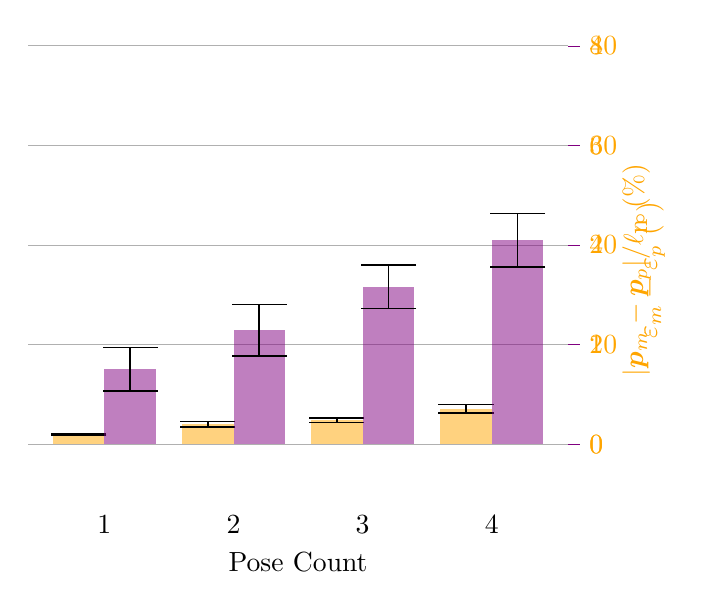
\begin{tikzpicture}
\definecolor{color0}{rgb}{1,0.647058823529412,0}
\definecolor{color1}{rgb}{0.501960784313725,0,0.501960784313725}
\begin{axis}[
anchor=origin,
axis line style={draw=none},
tick align=outside,
tick pos=both,
x grid style={white!69.01960784313725!black},
xmin=-0.59, xmax=3.59,
xtick style={color=black},
xtick style={draw=none},
xtick={0,1,2,3},
xticklabels={ , , , },
y grid style={white!69.01960784313725!black},
ylabel style={color=color0},
ylabel={\(\displaystyle |\bm{p}_m - \bm{p}_p|/\ell_{\textnormal{n}}\) (\%)},
ymin=-0.5, ymax=4,
ytick pos=left,
ytick pos=right,
ytick style={color=color0},
ytick style={color=color0},
yticklabel style={color=color0}
]
\draw[fill=color0,draw opacity=0,fill opacity=0.5] (axis cs:0,0) rectangle (axis cs:-0.4,0.101285450523065);
\draw[fill=color0,draw opacity=0,fill opacity=0.5] (axis cs:1,0) rectangle (axis cs:0.6,0.200585077887633);
\draw[fill=color0,draw opacity=0,fill opacity=0.5] (axis cs:2,0) rectangle (axis cs:1.6,0.24257866269063);
\draw[fill=color0,draw opacity=0,fill opacity=0.5] (axis cs:3,0) rectangle (axis cs:2.6,0.35771509777642);
\path [draw=black, semithick]
(axis cs:-0.2,0.0958446211739466)
--(axis cs:-0.2,0.106726279872183);
\path [draw=black, semithick]
(axis cs:0.8,0.172236179824473)
--(axis cs:0.8,0.228933975950793);
\path [draw=black, semithick]
(axis cs:1.8,0.219505438999105)
--(axis cs:1.8,0.265651886382156);
\path [draw=black, semithick]
(axis cs:2.8,0.316942720435514)
--(axis cs:2.8,0.398487475117325);
\addplot [semithick, black, mark=-, mark size=10, mark options={solid}, only marks]
table {%
-0.2 0.0958446211739466
0.8 0.172236179824473
1.8 0.219505438999105
2.8 0.316942720435514
};
\addplot [semithick, black, mark=-, mark size=10, mark options={solid}, only marks]
table {%
-0.2 0.106726279872183
0.8 0.228933975950793
1.8 0.265651886382156
2.8 0.398487475117325
};
\end{axis}
\begin{axis}[
anchor=origin,
axis line style={draw=none},
axis y line=right,
tick align=outside,
tick pos=both,
x grid style={white!69.01960784313725!black},
xlabel={Pose Count},
xmin=-0.59, xmax=3.59,
xtick style={color=black},
xtick style={draw=none},
xtick={0,1,2,3},
xticklabels={1,2,3,4},
y grid style={white!69.01960784313725!black},
ylabel style={color=color0},
ylabel={\(\displaystyle \varepsilon_m - \varepsilon_p\) (\(\displaystyle ^\circ\))},
ymajorgrids,
ymin=-10, ymax=80,
ytick pos=left,
ytick pos=right,
ytick style={color=color0},
ytick style={color=color1},
yticklabel style={color=color0}
]
\draw[fill=color1,draw opacity=0,fill opacity=0.5] (axis cs:0,0) rectangle (axis cs:0.4,15.0786819246887);
\draw[fill=color1,draw opacity=0,fill opacity=0.5] (axis cs:1,0) rectangle (axis cs:1.4,22.8768747230798);
\draw[fill=color1,draw opacity=0,fill opacity=0.5] (axis cs:2,0) rectangle (axis cs:2.4,31.6549558066518);
\draw[fill=color1,draw opacity=0,fill opacity=0.5] (axis cs:3,0) rectangle (axis cs:3.4,40.9901304230399);
\path [draw=black, semithick]
(axis cs:0.2,19.4499708840864)
--(axis cs:0.2,10.7073929652911);
\path [draw=black, semithick]
(axis cs:1.2,28.0575219565479)
--(axis cs:1.2,17.6962274896116);
\path [draw=black, semithick]
(axis cs:2.2,36.0367603405924)
--(axis cs:2.2,27.2731512727111);
\path [draw=black, semithick]
(axis cs:3.2,46.3371200454781)
--(axis cs:3.2,35.6431408006017);
\addplot [semithick, black, mark=-, mark size=10, mark options={solid}, only marks]
table {%
0.2 19.4499708840864
1.2 28.0575219565479
2.2 36.0367603405924
3.2 46.3371200454781
};
\addplot [semithick, black, mark=-, mark size=10, mark options={solid}, only marks]
table {%
0.2 10.7073929652911
1.2 17.6962274896116
2.2 27.2731512727111
3.2 35.6431408006017
};
\end{axis}
\end{tikzpicture}
%% End matplotlib2tikz content %% 
\end{document}